% !TEX root = thesis_draft.tex

\section{Prediction of task performance}

\subsection{Introduction}

We attempt to predict the performance of the dyads in
\textcite{newman_effects_2021}'s cooperation task based on inter-brain synchrony
(IBS) values and the amplitude of the P3 event-related potential (ERP)
component. There are many potential mechanisms that could cause IBS and
simultaneously be predictive of task performance. For example, functional
similarities could arise in the neural oscillations as a result of participants
placing themselves in their partner's shoes (i.e., theory of mind).
Alternatively, performing the same strategy could lead to similar brain
activity, as could focussing on the same (if chosen automatically correct)
stimulus. In the end, while the exact mechanism is interesting from a
theoretical point of view, it does not matter when the goal is to predict task
performance. Instead, it would be a possible follow-up question.

The P3 ERP component, also known as the P300 component
\parencite[p.~5]{luck_introduction_2014}, is a positive deflection in an EEG
signal about 300ms after a stimulus is shown
\parencite{sutton_evoked-potential_1965}. It generally occurs as a response to
infrequent but task-related stimuli \parencite{polich_neuropsychology_2011}.
The mechanism underlying the P3 is unclear, but the most popular theory is the
\textit{context updating model} \parencite[p.~96]{luck_introduction_2014}. It
explains the P3 as a consequence of updating the neural representation of the
environment when the stimulus (unexpectedly) changes
\parencite{polich_neuropsychology_2011}. The P3 decreases during mind-wandering
\parencite{jin_predicting_2019}. In \textcite{newman_effects_2021}'s
task the context is a bit more complex than frequent or infrequent stimuli being
shown: participants instead need to reason about how the other participant is
choosing one of the four stimuli. But this still requires keeping track of
choices, feedback and hypotheses. It is not out of the question this also
would evoke a context updating P3 ERP. Alternatively, negative feedback could be
surprising in itself when the participant believes to have hit upon a `shared
rule' on how to perform the task.

We consider a number of classification methods: logistic regression \parencite[p.137]{goodfellow_deep_2016}, support
vector machines \parencite[p.137--139]{goodfellow_deep_2016}, random decision
forests \parencite{tin_kam_ho_random_1995} and multi-layer perceptrons
\parencite{rumelhart_learning_1987}. We attempt both across-session and
within-session prediction.

\subsection{Methods}

\begin{figure}[!htpb]
  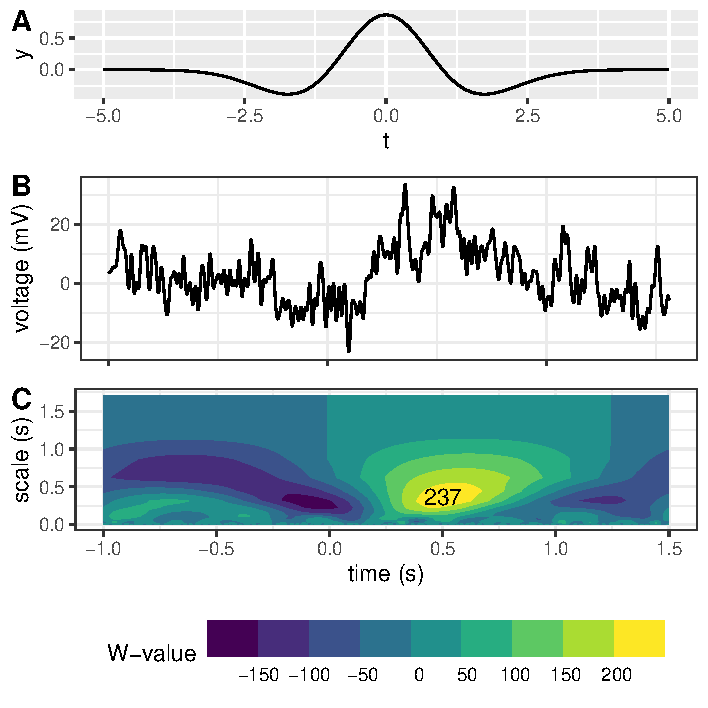
\includegraphics[width=\linewidth]{../stats/results/cwt.pdf}
  \caption{When applying the continuous wavelet transform using the mexican hat template $\psi(t)$ in (A) to an example trial $f(t)$ in (B) we obtain (C). The local maximum in (C) is shown and is our single-trial ERP measure. (B) is identical to Figure~\ref{fig:freqanalysis}A.}
  \label{fig:cwt}
\end{figure}
  
The methods of the prediction task are based on those of a study by
\textcite{jin_predicting_2019}.

Because EEG data contains a lot of noise, ERP components are normally identified
by averaging over multiple trials \parencite[p.~259]{luck_introduction_2014}.
This is not feasible when predicting task performance, as we need to predict
whether the dyad guessed correctly for each trial. Instead, we use a method that
attempts to match each trial's EEG signal with the shape of a template. The
template $\psi(t)$ takes the form of an idealized ERP component (see
Figure~\ref{fig:cwt}A). This function, sometimes called `mexican hat', is
defined as follows \parencite{bostanov_t-cwt_2006}:
\begin{equation}
\psi(t) = (1 - 16t^2)e^{-8t^2}.
\end{equation}

The method we use, which is devised by \textcite{bostanov_recognition_2004},
uses a continuous wavelet transform (CWT) to calculate the covariance between
the signal and the template at different time points and for different template
scales. The CWT is defined as \parencite{bostanov_t-cwt_2006}:
\begin{equation}
W(s, t) = \cfrac{1}{\sqrt{s}}\int\displaylimits_{-\infty}^\infty f(\tau) \cdot \psi\left(\frac{\tau - t}{s}\right) d\tau
\end{equation}
where $f(t)$ is the signal that is transformed, $s$ scales the template
$\psi(t)$ and $\tau$ shifts the template. See for an example signal
Figure~\ref{fig:cwt}B, and for a corresponding example CWT output
Figure~\ref{fig:cwt}C.

The single-trial P3 ERP is defined as the local maximum in $W(s, t)$ between
$t=250\text{ms}$ and $t=600\text{ms}$ \parencite{jin_predicting_2019}.

\begin{table}[!htbp]
\caption{Thirty sessions were randomly assigned to the train set, eight to the test set.}
\label{tab:predictionsplit}
\begin{tabularx}{\linewidth}{l X}
  \hline
  assignment & session numbers\\\hline
  train set & 2, 3, 4, 6, 8, 9, 10, 11, 12, 13, 14, 16, 18, 19, 21, 22, 23, 24, 25, 27, 29, 31, 33, 35, 36, 37, 38, 39, 41, 42\\
  test set & 5, 7, 15, 17, 20, 28, 30, 40\\\hline
\end{tabularx}
\end{table}

The data set was randomly split into a train- and a test set
(see Table~\ref{tab:predictionsplit}). The latter was not accessed during training and only used for
final model evaluation. Such a test set is sometimes also called a lock box
\parencite{hosseini_i_2020}.

Because on average dyads are correct a bit more than they are incorrect, we use
random oversampling during training to account for this imbalance in the data
set \parencite{maimon_data_2005}. Otherwise, a model that classifies every
example as correct would result in an accuracy higher than 50\%, which is not
helpful when determining whether IBS measures and the P3 component can predict
task performance.

For each trial, the three IBS measures where calculated in both the alpha and
theta band. Additionally, single-trial P3 ERP components were calculated for
both participants. These eight calculations were all repeated 32 times for each
electrode, resulting in a total of 256 features.

Phase locking value values were normalized using the inverse cumulative
density function of the normal distribution. Circular correlation and
imaginary part of coherency values were Fisher-transformed. All
single-trial ERP trials were log-transformed. This was impossible for (a trivial
amount of) negative values, which were capped at 0.05 before the transformation.
All the resulting values were additionally z-transformed.

We report sensitivity, specificity and balanced accuracy. Sensitivity looks at
correct trials. It tells us what proportion of those the classifier predicted to
be correct \parencite{yerushalmy_statistical_1947}. Specificity looks at the
incorrect trials. It tells us what proportion of those the classifier predicted
to be incorrect \parencite{yerushalmy_statistical_1947}. Balanced accuracy
is the mean of the two. Classifiers were trained to maximize balanced accuracy.

During training, 10-fold cross validation was used. Folds were chosen such that
data of a single session did not leak into both a train and validation set,
as this could potentially lead to overoptimistic accuracy estimates.

Random hyperparameter search was used \parencite{bergstra_random_2012} for 30
iterations, with hyperparameters sampled from log uniform distributions with the
exception of the random forest integer hyperparameter values, were a discrete
uniform distribution was used instead.

For the logistic regression classifier, which served as a baseline, the L1 norm
was used as it forces unused features to be dropped entirely. We optimized the
regularization strength hyperparameter $C$
\parencite[also known as \textit{capacity};][p.~117]{goodfellow_deep_2016}.

For the support vector machine, a radial basis function was used. We optimized
its radius ($\gamma$) and regularization ($C$) hyperparameters. As the SVM
performed best in earlier EEG prediction tasks
\parencite{jin_predicting_2019,lotte_review_2007}, we used it for two variations
on the experiment as well. An SVM was trained without P3 ERP component data
(i.e. taking 192 features as its input), and 256 SVMs were trained that only
took a single feature each to determine the relative importance of features. For
these variations, hyperparameter values of the main experiment were used.

Two hyperparameters were optimized for the random forest classifier. Amount of
trees (1--250) and maximum amount of features (1--30). For the multi-layer
perceptron, a fixed architecture consisting of a single hidden layer of 10
neurons was used. The ReLU function, i.e.
\begin{equation}
f(x) = \max(0, x)
\end{equation}
was used as activation function. The learning rate (alpha) was optimized.

Finally, some within-session and within-condition classification was attempted
using SVM classifiers. This results in small data sets of ~90 rows, which were
split in train sets containing ~75\% of the rows and test sets containing ~25\%.
Hyperparameter optimization was the same as in the `main' prediction experiment,
except for the choice of cross-validation folds. There were no groups to take
into account, instead folds were kept balanced such as to have both `correct'
and `incorrect' examples. A dimension reduction step using principal component
analysis (PCA) was added to better cope with the small amount of available data.
The amount of components $k$ was optimized using cross-validation.

\begin{verbatim}
\end{verbatim}

\subsection{Results}

The outcome of the cross-validation procedure used to determine the
hyperparameters was visualized in a number of parameter vs. test performance
plots. These plots can be found in Appendix~\ref{app:supplementaryfigures} for
logistic regression (Figure~\ref{fig:learning_curve_logistic}), for the SVMs
(Figure~\ref{fig:learning_curve_svm}), for the Random Forest classifier
(Figure~\ref{fig:learning_curve_rf}), for the multi-layer perceptron
(Figure~\ref{fig:learning_curve_mlp}) and finally for the within-session SVM
(Figure~\ref{fig:learning_curve_within_dyad}).

\subsubsection{Evaluation}

\begin{figure}[!htpb]
  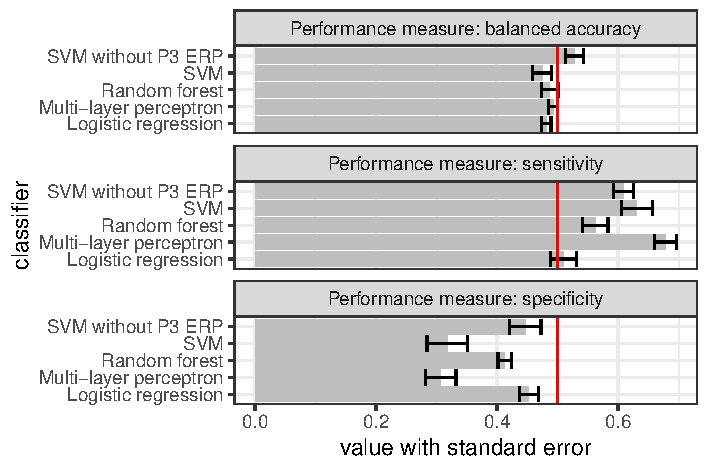
\includegraphics[width=\linewidth]{../stats/results/evaluation_avg.pdf}
  \caption{Mean classification performance on the test set for different performance metrics.}
  \label{fig:evaluation_avg}
\end{figure}

\begin{figure}[!htpb]
  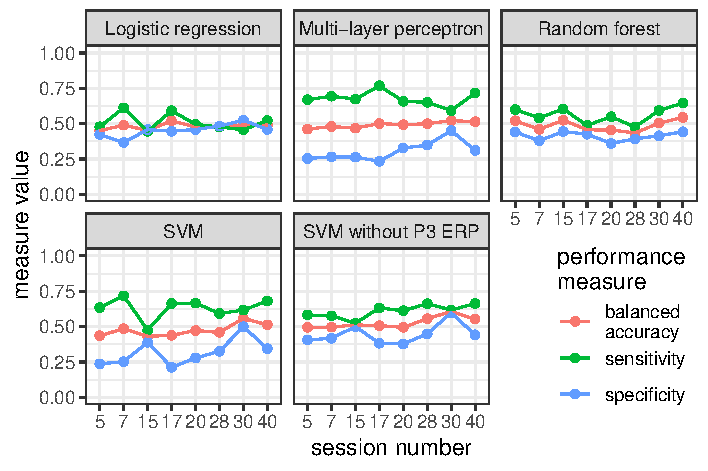
\includegraphics[width=\linewidth]{../stats/results/evaluation_detail.pdf}
  \caption{Classification performance for each test set session. (Detailed version of Figure~\ref{fig:evaluation_avg}).}
  \label{fig:evaluation_detail}
\end{figure}

Figure~\ref{fig:evaluation_avg} shows that classification performance, as
measured using the balanced accuracy, is at chance level (i.e. 0.5) for all
classifiers. Although it might seem like some error bars do not overlap with
0.5, this would be the case if confidence intervals were shown instead of
standard errors, as those are almost two times as big.
Figure~\ref{fig:evaluation_avg} also suggests that an SVM classifier that was
not trained on P3 ERP component-based features outperforms an SVM classifier
that was.

We see that all classifiers have a higher sensitivity than specificity. In other
words, the classifiers are better at predicting correct trials as correct than
incorrect trials as incorrect. This would make sense if we had not corrected for
the imbalance in the data, but between the balanced accuracy performance measure
and the random oversampling process, that is not the case. Apparently, the
classifiers converge on a (slight) bias to predict trials to be correct
regardless. This is not the case for all sessions, as can be seen in
Figure~\ref{fig:evaluation_detail}. Also, the logistic regression classifier
seems to show this phenomenon less strongly.

\subsubsection{Important features}

\begin{figure}[!htpb]
  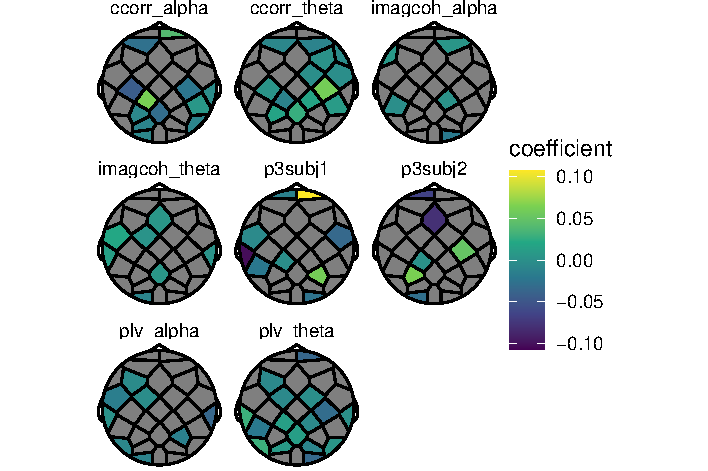
\includegraphics[width=\linewidth]{../stats/results/logistic_coef.pdf}
  \caption{Logistic regression (L1 norm): coefficients for each feature. Missing data  (grey background) means the feature was dropped by the classifier completely. Features with coefficients further from zero have a greater influence on the final prediction. Synchrony measures (ccorr = circular correlation, imagcoh = imaginary part of coherency, plv = phase locking value) were calculated for both the alpha and theta band. Both subjects contribute a P3 single-trial ERP value.}
  \label{fig:logistic_coef}
\end{figure}

The final logistic regression model drops most predictors, and puts the highest
importance on P3 ERP component features (see Figure~\ref{fig:logistic_coef}).
This is likely to be a fluke, as we would expect an actual pattern to be
duplicated among P3 ERP components for both subjects. Otherwise, no pattern is
discernible, which is what we would expect for a model that predicts at chance
level.

\begin{figure}[!htpb]
  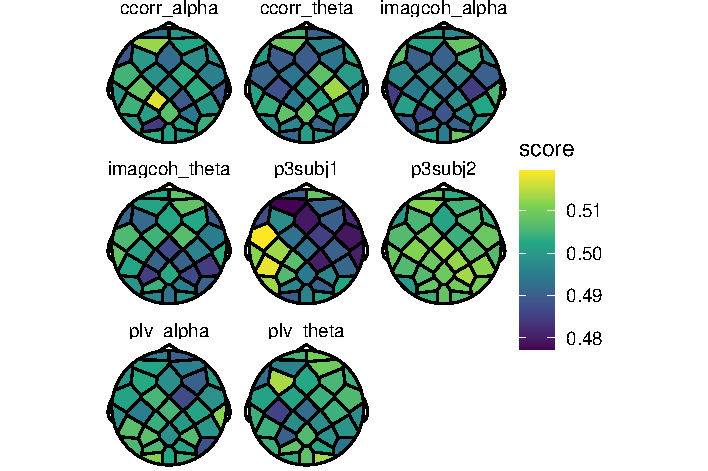
\includegraphics[width=\linewidth]{../stats/results/svm_indiv_topo.pdf}
  \caption{Balanced accuracy of SVMs trained on single features, averaged over sessions. Synchrony measures (ccorr = circular correlation, imagcoh = imaginary part of coherency, plv = phase locking value) were calculated for both the alpha and theta band. Both subjects contribute a P3 single-trial ERP value. Outliers lie further than 1.5 inter-quartile ranges from the hinge.}
  \label{fig:svm_indiv_topo}
\end{figure}

\begin{figure}[!htpb]
  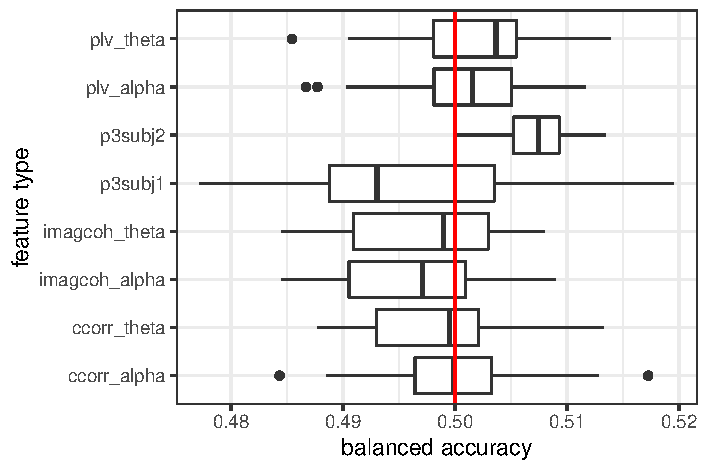
\includegraphics[width=\linewidth]{../stats/results/svm_indiv.pdf}
  \caption{Balanced accuracy of SVMs trained on single features, averaged over electrodes and sessions. A box plot summary of the data shown in Figure~\ref{fig:svm_indiv_topo}.}
  \label{fig:svm_indiv}
\end{figure}

Another way of assessing the importance of individual features in predicting
task performance is to look at the balanced accuracy of the SVMs that were
trained on single features (see Figure~\ref{fig:svm_indiv_topo}). In general,
these classifiers also perform at around chance level. There is a bit more
variation in perfomance of the classifiers that were trained on P3 ERP
components of the first participant compared to the other classifiers (see
Figure~\ref{fig:svm_indiv}). As this matches our findings using the logistic
regression classifier with L1 norm, it is likely to be caused by a pattern in
the P3 ERP component data and not just by a classifier induced artifact. But as
the pattern is again not reproduced for the second participant, it is unlikely
it contributes to predicting task performance.

\subsubsection{Within-session classification}

\begin{figure}[!htpb]
  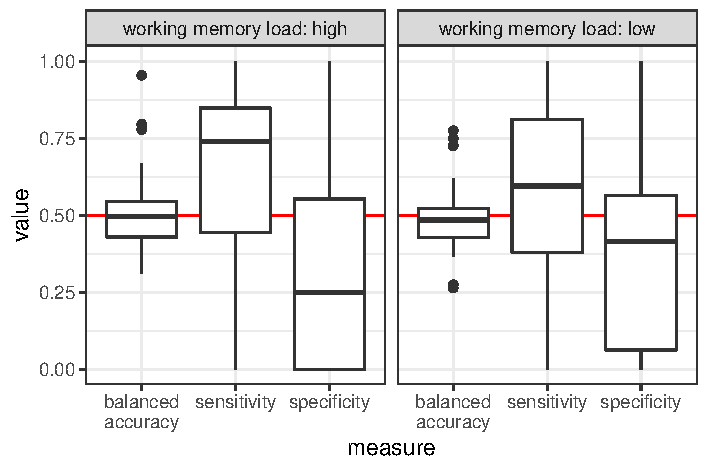
\includegraphics[width=\linewidth]{../stats/results/within_dyad_summary.pdf}
  \caption{Within-session classification performance on the test set (box plot, outliers lie further than 1.5 inter-quartile ranges from the hinge).}
  \label{fig:within_dyad_summary}
\end{figure}

\begin{figure}[!htpb]
  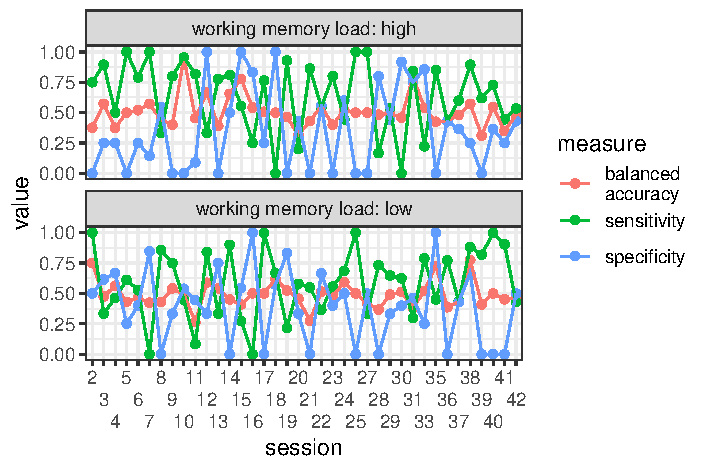
\includegraphics[width=\linewidth]{../stats/results/within_dyad_detail.pdf}
  \caption{Within-session performance on the test set (raw metrics, see Figure~\ref{fig:within_dyad_summary}) for summarized numbers.}
  \label{fig:within_dyad_detail}
\end{figure}

When predicting task performance within sessions for both low and high working
memory load, we see the same pattern as for the between-session classifiers.
Performance is still at chance level, and classifiers have on average higher
sensitivity than specificity (see Figure~\ref{fig:within_dyad_summary}).

When looking at the raw data in Figure~\ref{fig:within_dyad_detail}, we see
more variation (cf. Figure~\ref{fig:evaluation_detail}). But this is to be
expected as the test sets are much smaller.

\subsection{Discussion}

Prediction of task performance based on IBS values and single-trial
P3 ERP component values failed. There are two possible explanations for this.
It could be that another classification method would perform better. But as
different classifiers, classification scenarios and hyperparameters were tried,
another method is unlikely to yield wildly different results. The more likely
explanation is that there is simply not enough information in
IBS values and single-trial P3 ERP components to be able to predict task
performance. That would also be in line with the null results found in the time
course analysis and permutation test analysis described in this report.

While most classifiers had higher sensitivity than specificity, this was not the
case for the logistic regression classifier (see
Figure~\ref{fig:evaluation_detail}). Possibly, this is because it is one of the
more constrained models from a theoretical point of view, having a smaller
representational capacity \parencite[p.~110]{goodfellow_deep_2016}.

Interestingly, an SVM trained only on IBS values seems to perform slightly
better than one trained also on P3 ERP components. The difference is small, so
it could just be due to variation in the data. But an alternative explanation
worth considering is the \textit{curse of dimensionality}: because the data set
is relatively small compared to the amount of features, models are not
constrained all that much by the training examples
\parencite[p.~151--152]{goodfellow_deep_2016}. Leaving out features that do not
contribute much is helpful as a result. But there are other ways to constrain
classifiers. One is to force them to model the underlying distribution smoothly,
e.g. using regularization. This was the case for all discussed classifiers.
Another is to pre-process the data using a dimension reduction technique. This
approach was used for the within-session classifiers, which included a PCA step.
But that did not yield better classifiers.

The attempt to identify the most influential values in the classification
process was largely stymied by the lack of classifiers performing above chance
level. It suggests the first participant's P3 ERP component values might be more
influential. One possible explanation for that could be that the ERP component
features stand out because their distribution is the furthest from a normal
distribution. This could lead them to have an oversized effect on the models.
Negative ERP values being set to a fixed value, especially, introduces a few
(rare) outliers. Negative single-trial ERP values are rare and suggest errors in
the data cleaning, but in practise they are hard to avoid as getting rid of them
all would also throw out a lot of good data of other electrodes.

It is unlikely the first participant's P3 features are influential because they
actually help classification. In that case, we would expect them to also show up
in the P3 features for the second participant. Also, we would expect features
close to the midline to be more influential, as that is where the P3 effect is
strongest \parencite{polich_neuropsychology_2011}. Neither is the case (see
Figures~\ref{fig:logistic_coef} and~\ref{fig:svm_indiv_topo}).

Finally, a few notes. The use of balanced accuracy instead of normal accuracy is
important, as random oversampling is only used during training, not during
testing. Originally, I overlooked this, and in this case, it lead to models that
only predict a single outcome. This only became clear after looking at the
sensitivity and specificity measures. Random oversampling works well, but it can
lead to overfitting \parencite{maimon_data_2005}. Especially if the imbalance in
the data is big, it is worth considering more sophisticated methods to construct
balanced samples \parencite[][e.g. SMOTE]{maimon_data_2005}.

While performing within-session classification can profit from dyad-specific
signals that predict task performance in IBS and P3 values, it comes at a cost
of having only very little data available. In some test sets, no examples of
both correct and incorrect trials were available. This made it impossible to
train a classifier in a couple of cross-validation folds, and is also a cause of
the large variance in Figure~\ref{fig:within_dyad_detail}. The lack of data also
means that we have no choice but to randomly sample cross-validation folds from
the train set instead of respecting their causal ordering in time. When the
underlying time series is autocorrelated, as is not unlikely in EEG-derived
data, this could lead to overoptimistic predictions.
